%\noindent
\justifying
\setlength{\parskip}{1em}

This chapter focuses on improving the understanding of the fundamental concepts required to understand this thesis. Section \ref{GenerativeAdversarialNetworks} describes architecture of \acp{GAN}. Section \ref{CNNs} describes neural network layers, namely, convolution layer, activation layer, pooling layer and fully connected layer.


\section{Generative Adversarial Networks (GANs)}\label{GenerativeAdversarialNetworks}

\begin{figure}[H]
        \begin{center}
	    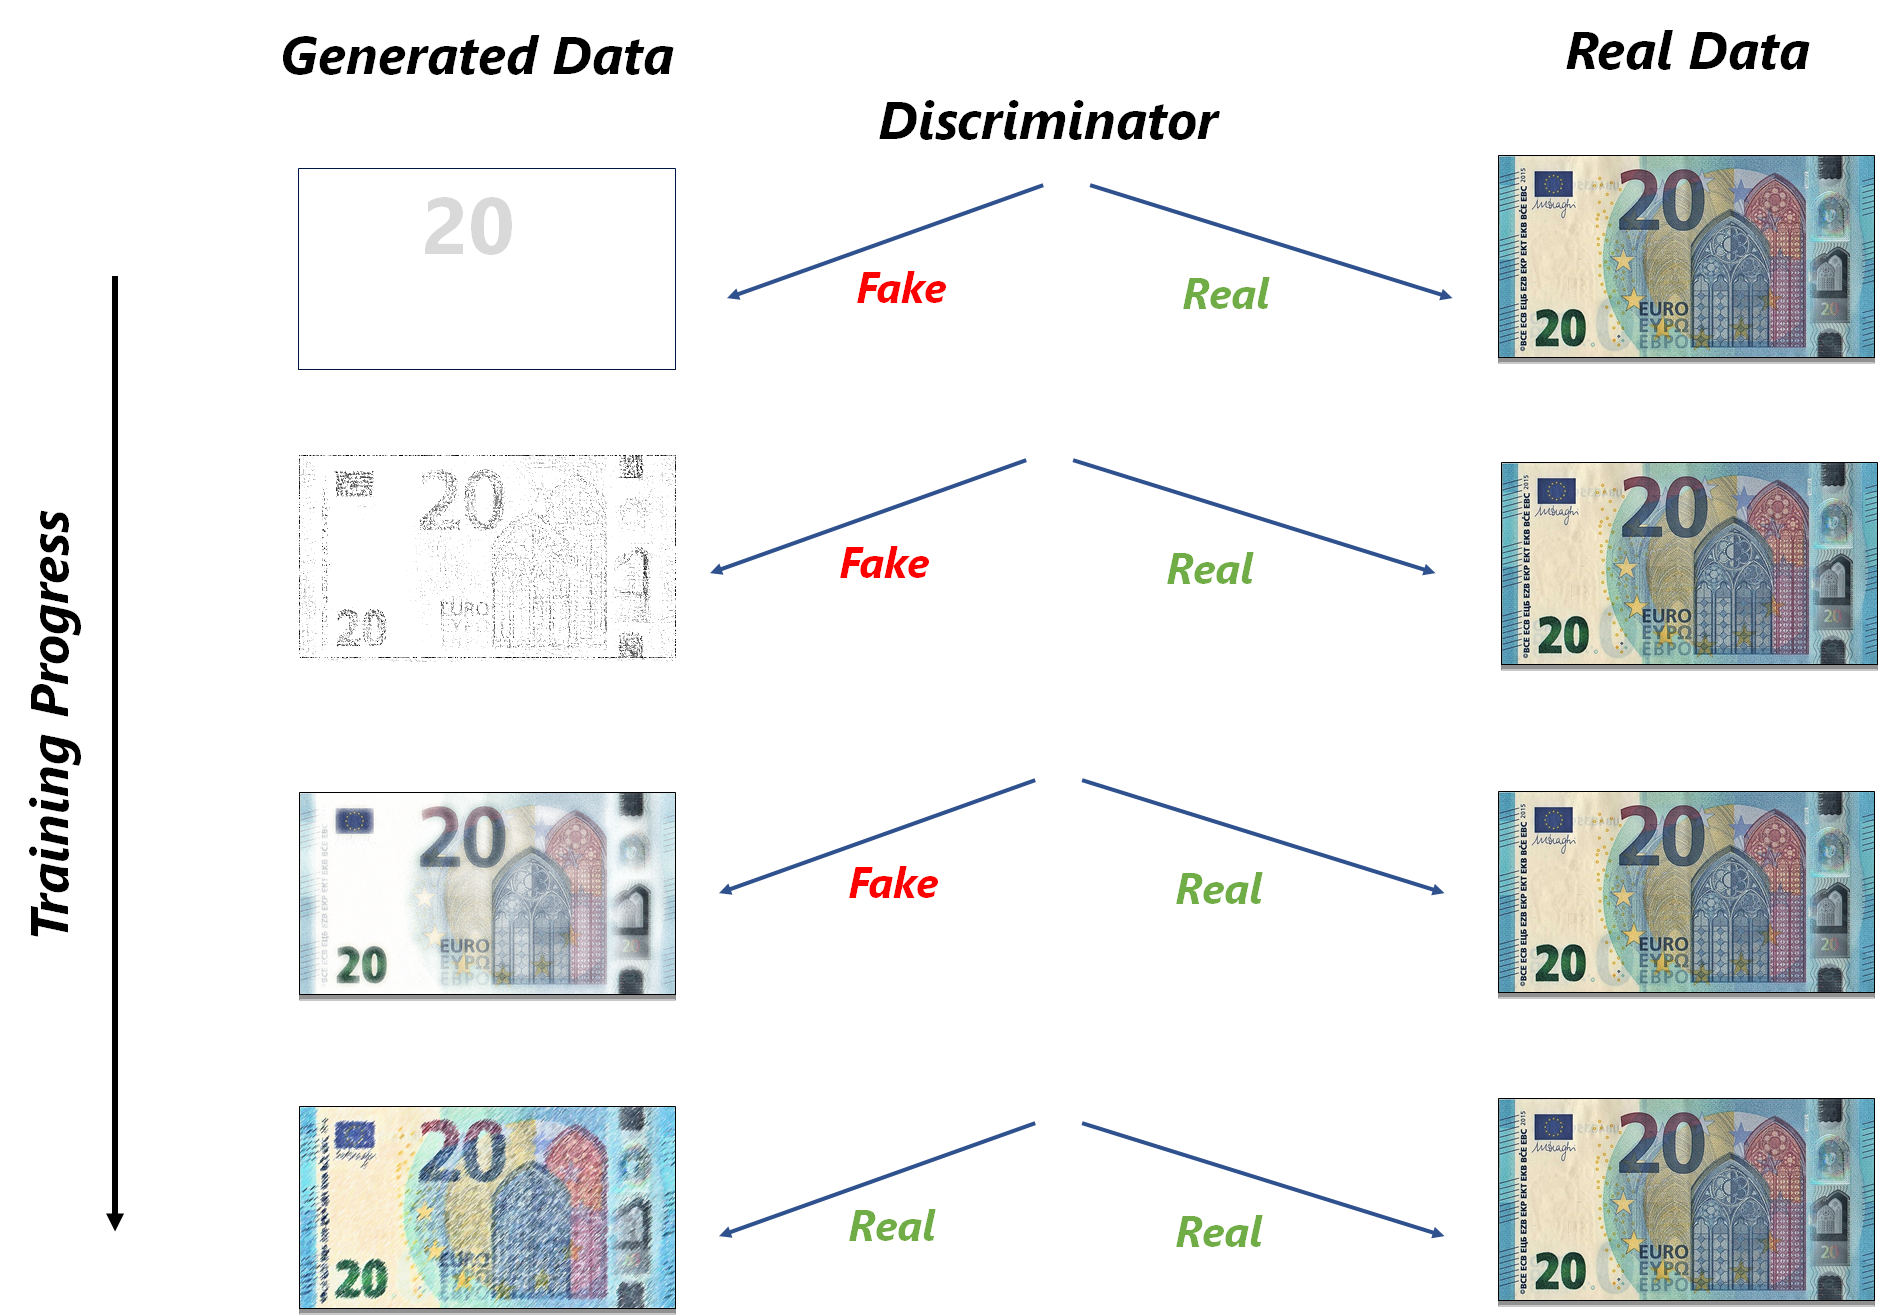
\includegraphics[scale=0.30]{images/Fundamentals/GANTrainingintuition.png}
	    \caption[Intuitive example of \ac{GAN} training progress.]{Intuitive example of \ac{GAN} training progress.}
	    \label{fig:GANTrainingintuition}
	    \end{center}
\end{figure}

% Both generator and discriminator are trained simultaneously. 
%, the multilayer perceptron can loosely be indicated by \acp{ANN}

\acp{GAN} have two models in their architecture first is the generator and the second is the discriminator and both models can be implemented using multilayer perceptrons \cite{goodfellow2014generative}. Let's try to understand the function of \acp{GAN} intuitively. Consider generator is a forger who creates fake currencies, with the intention of making them realistic as much as possible. Further, the discriminator is an expert who distinguishes forged and real currencies. The discriminator has access to images generated by the generator and real images present in the dataset. The generator generates fake images without having access to the real images using random noise distribution. The discriminator learns by the feedback error after misclassifying real images as fake and fake images as real. The generator also learns by the feedback error given by the discriminator, after it successfully classifies image produced by the generator as fake. To produce a better quality of fake images, the generator model is updated using the feedback error given by the discriminator. It is a setup where both generator and discriminator are competing with each other. An intuitive example of \ac{GAN} training process is illustrated in figure \ref{fig:GANTrainingintuition}. It depicts, during the initial stages of the training, the generated images by the generator are easily distinguished as fake by the discriminator. After training iterations, the quality of the generated images by the generator increases. The generator learns using feedback error given by the discriminator. Finally, the generator learns to produce realistic images and the discriminator starts to classify them as real.

Now, let's have a look into the \ac{GAN}'s architecture. As described earlier, the task of the \ac{GAN} is to generate fake samples that are realistic. The training dataset of real data samples $S$ serves as an input to the discriminator $D$. The random noise vector $Z$ retrieved from the random noise distribution serves as an input to the generator $G$ to produce fake samples. The generator $G$ takes $Z$ as an input and outputs a fake sample $S'$. Its goal is to create fake samples that are realistic as much as possible and indistinguishable from the real samples from the training dataset. The discriminator $D$ takes input from real data sample $S$ that are present in the training dataset and fake samples $S'$ generated from the generator $G$. For each sample, it determines and outputs the probability of the sample that is real. For every discriminator's prediction, the classification error is backpropagated to update both generator and discriminator during iterative training. The discriminator's weights are updated to maximize classification accuracy which means, maximizing the probability of correct prediction $S$ as real and $S'$ as fake. The generator's weights are updated to produce quality samples and maximize the probability that the discriminator makes mistake and misclassifies $S'$ as real. \ac{GAN} in action is illustrated in figure \ref{fig:GANStructure}.


%The training dataset has a set of real data samples, from which the generator learns to create fake samples that are similar to the real samples
%Also, the discriminator gets smarter and smarter over time, to distinguish fake images and real images, like mentioned earlier both models are trained simultaneously. But at a certain point generator starts to produce realistic images which the discriminator classifies as real. 
%The discriminator learns by the error signal provided by the ground truth of distinguishing whether the image came from the dataset of real images or from the generator. The generator learns using the same error signal given by the discriminator to produce a better quality of forged or fake images. It is a setup where both generator and discriminator are competing with each other.


\vspace*{0.4cm}
\begin{figure}[H]
        \begin{center}
	    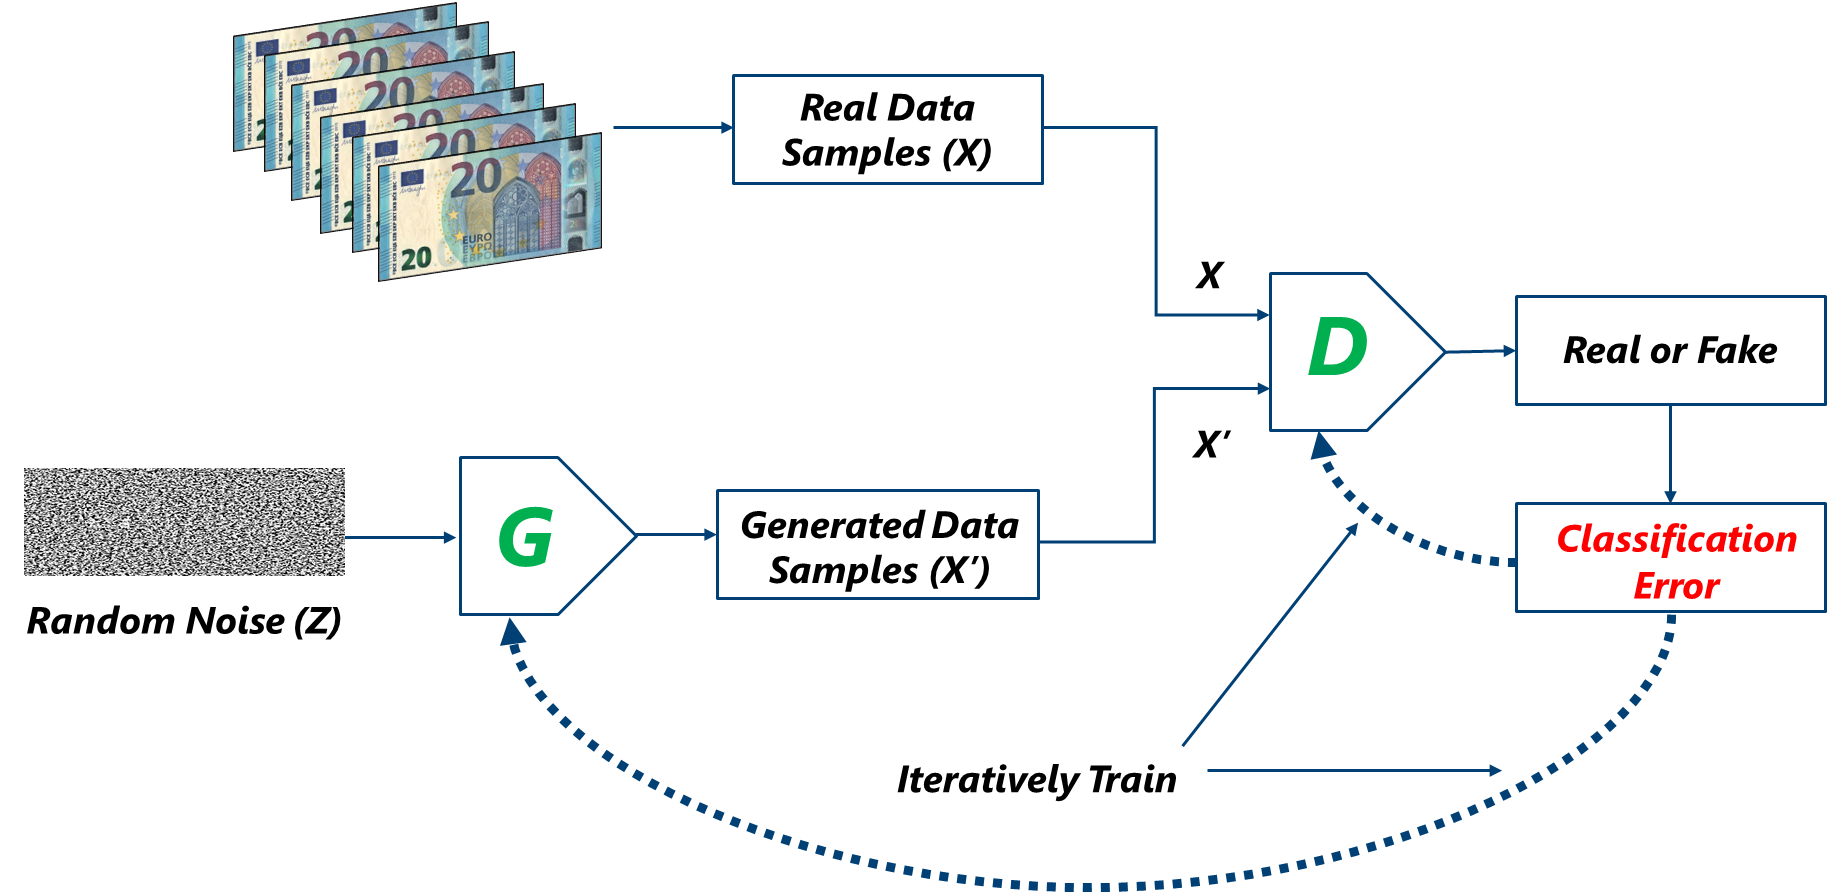
\includegraphics[scale=0.30]{images/Fundamentals/GANStructure.png}
	    \caption[An illustration of \ac{GAN} architecture.]{An illustration of \ac{GAN} architecture along with the generator's and discriminator's inputs, outputs and their interactions.}
	    \label{fig:GANStructure}
	    \end{center}
\end{figure}


%In practice, the discriminator is may not be trained till it is optimal \cite{Creswell_2018}.

Let's try to understand the mathematics behind \acp{GAN}. For learning the generator’s distribution $p_g$ over data $x$, the input noise variable defined as $p_z(z)$. The generator $G$ and discriminator $D$ are the differential functions. They are represented by multilayer perceptrons with parameters $\theta_g$ and $\theta_d$ respectively \cite{goodfellow2014generative}. The mapping function from some representation space, called, the latent space to the space of data, is represented by $G(z; \theta_g)$. The $D(x; \theta_d)$ maps data $x$ to the probability that it came from the real data distribution rather than generator distribution $p_g$. Basically, $D(x)$ represents the likelihood of $x$ came from the data rather than $p_g$. $D(x; \theta_d)$ outputs a single scalar value between $[0,1]$. $D$ is trained to maximize the probability of correctly labeling both training examples and data generated by the $G$. Usually, when the generator is training, the discriminator does not train and vice versa. For a fixed $G$, the discriminator is trained to classify data as either being from the real data distribution (real, probability close to one) or from the fixed generator(fake, probability close to zero). After a certain number of training iterations, when the discriminator is optimally optimized, it can be fixed and the generator $G$ advances to learn by the error provided by the discriminator to produce plausible data. At the end of the training, if the generator can match the real data distribution, then the discriminator is maximally confused, will predict 0.5 probability for its inputs and mathematically $G$ is being trained to minimize $log(1 - D(G(z))$. It can be said $D$ and $G$ compete with each other just like a two-player minimax game to achieve the objective $\mathcal{L}_{GAN}(G, D)$:


\begin{equation}\label{ganObjectiveFunction}
\underset{G}{\min}\ \underset{D}{\max}\ \mathcal{L}_{GAN}(D, G) = E_{x\sim p_{data}(x)}[log D(x)] + E_{z\sim p_z(z)}[log(1 - D(G(z)))].
\end{equation}


Authors mentioned, in practice, the equation \ref{ganObjectiveFunction} may not give enough gradient for $G$ to learn well. During early in learning phase, when $G$ is poor, $D$ can reject samples with high confidence because they are clearly distinct from the training data. In this case, term $log(1 - D(G(z)))$ in equation \ref{ganObjectiveFunction} saturates very quickly \cite{goodfellow2014generative}. Hence, Authors proposed to train $G$ to maximize $log D(G(z))$ rather than training it to minimize $log(1 - D(G(z)))$. This modified objective function leads to the same fixed point of the dynamics of $G$ and $D$ by providing much stronger gradients early in learning \cite{goodfellow2014generative}. The \ac{GAN} converging to match generated data distribution $p_g$ to real data distribution $p_{data}$ is illustrated in the figure \ref{fig:GANTraining}.

\begin{figure}[H]
        \begin{center}
	    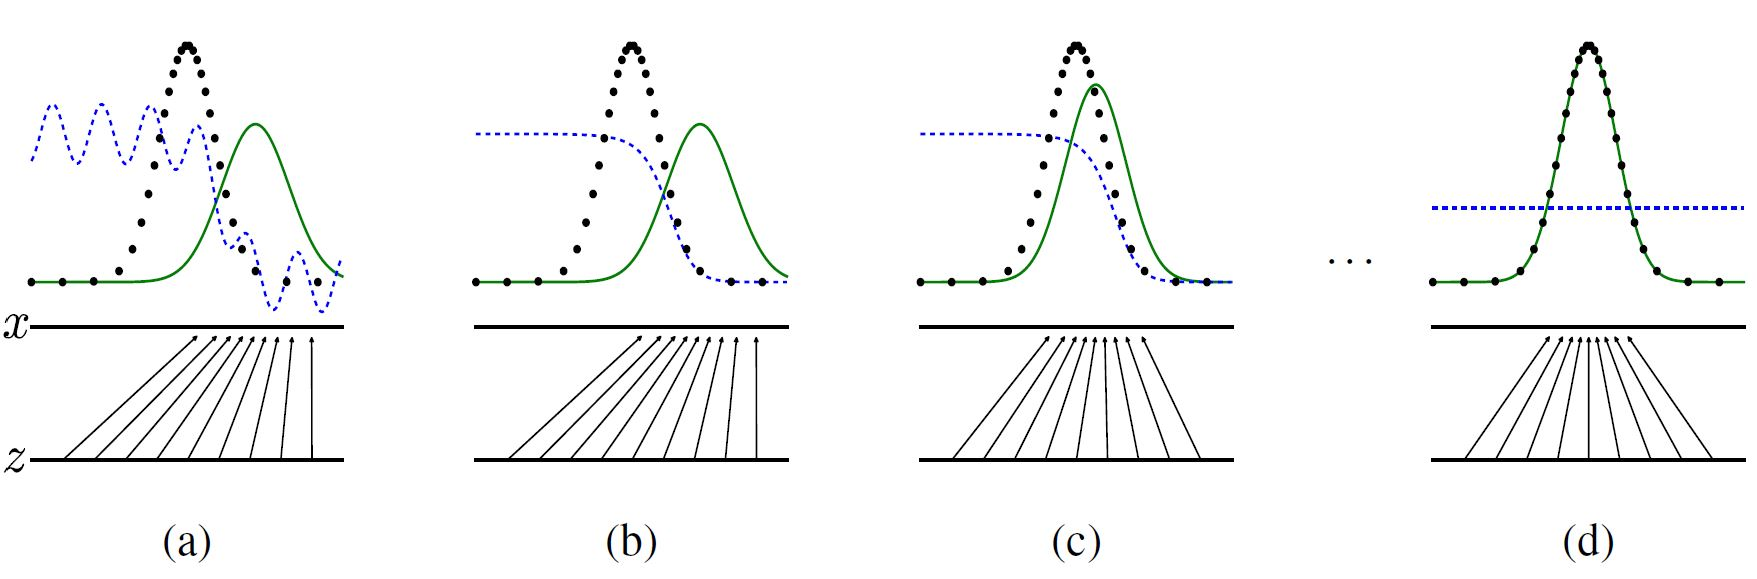
\includegraphics[scale=0.49]{images/Fundamentals/GANTraining.jpg}
	    \caption[An illustration of \ac{GAN} converging to match generated data distribution $p_g$ to real data distribution $p_{data}$.]{An illustration of \ac{GAN} converging to match generated data distribution $p_g$ to real data distribution $p_{data}$. While training \acp{GAN}, discriminative distribution is simultaneously updated so it will discriminate or distinguish samples from the real data distribution $p_x$ from those of the generated data distribution $p_g$. In the figure, the discriminative distribution is represented by ($D$, dashed line, blue), the real data distribution $p_x$ represented by (dotted line, black) and the generated data distribution $p_g$ represented by (G, green, solid line).
	    
	    
	    
	    
	    
	    
	    
	    The lower horizontal line represents the domain of noise distribution $p_z$ from which $z$ is sampled uniformly. The horizontal line above represents the part of the domain of real data $x$. The upward arrows depict the mapping of $x = G(z)$, which creates the non-uniform generated data distribution $p_g$ on transformed samples. (a) Consider, $G$ and $D$ are on the verge of convergence, $p_g$ is almost similar to $p_{data}$ and $D$ is a partially accurate classifier. (b) Slowly, $D$ is trained further to distinguish real data samples from generated data samples. For a fixed $G$, there is an optimal discriminator, $D^*(x) = \frac{p_{data}(x)}{p_{data}(x) + p_g(x)}$. (c) The $G$ is updated using gradients that are backpropagated from $D$ and makes $G(z)$ to flow into the regions that are most probably classified as real data, the parameters of the $G$ are updated, while the parameters of the $D$ are fixed. (d) After several steps of training, $G$ is optimal where $p_g = p_{data}$, which is equivalent to the optimal $D$ predicting 0.5 for all samples drawn from $x$, at this stage $D$ is maximally confused and will not able to distinguish real data samples from generated data samples, i.e. $D(x) = \frac{1}{2}$ \cite{goodfellow2014generative}.}
	    \label{fig:GANTraining}
	    \end{center}
\end{figure}

\subsection{\ac{GAN} Training}

% In figure \ref{fig:generatorAndDiscriminatorTraining} shows the same \ac{GAN} network in different stages of the training process at distinct time points.

This section discusses the training algorithm of the \ac{GAN}. The training algorithm is divided into two sections. These two sections are discriminator training and generator training. It illustrates the discriminator and generator training process together. It also illustrates, while training the generator, the discriminator is not training, basically, it means, a fixed discriminator is used while training the generator. Hence, the training dataset of real data samples is grayed out in the section where the generator training is illustrated, and while training discriminator both generated samples from the generator and real samples are used as an input. In the following sections generator's and discriminator's training process is described along with intuitive figures. Further, the \ac{GAN} training algorithm has been described in the form of pseudo-code. The algorithm of the \ac{GAN} is pictorially illustrated in the figure \ref{fig:generatorAndDiscriminatorTraining}

\subsubsection{Discriminator Training}\label{TheDiscriminatorSubSection}

In \acp{GAN}, the discriminator is a binary classifier. It attempts to classify real data samples from fake data samples generated by the generator. It provides the likelihood that its input is a real data sample. In computer vision tasks, the discriminator classifies images, hence, it is implemented using \ac{CNN} \cite{radford2016unsupervised}. The discriminator's training data come from the two resources, training dataset or collection of real data samples and fake data samples generated by the generator. The discriminator is penalized for misclassifying a real data sample as fake or a fake data sample as real, such classification error is called discriminator loss. The weights of the discriminator network are updated using backpropagated discriminator loss. The training process of the discriminator $D$ using backpropagation illustrated in figure \ref{fig:discriminatorTraining}.

%The discriminator can be implemented using a multilayer perceptron which is suitable to the kind of data it's classifying. 
%During \ac{GAN} training, the discriminator is trained by both real data samples and fake data samples generated by the generator.

\vspace*{0.2cm}
\begin{figure}[H]
        \begin{center}
	    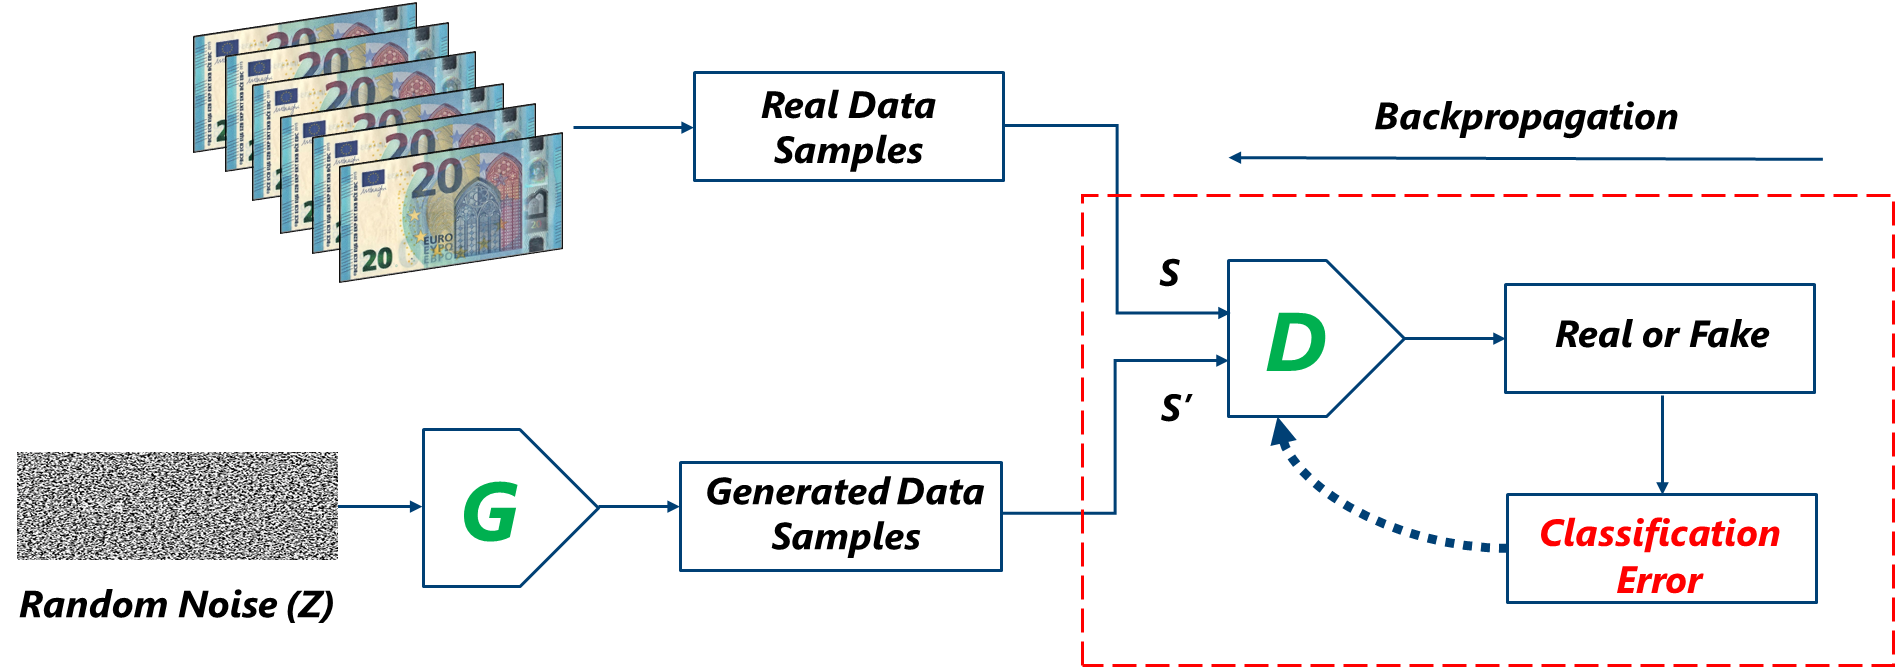
\includegraphics[scale=0.30]{images/Fundamentals/discriminatorTraining.png}
	    \caption[An illustration of the training of the discriminator $D$ using backpropagation.]{An illustration of the training of the discriminator $D$ using backpropagation.}
	    \label{fig:discriminatorTraining}
	    \end{center}
\end{figure}

\subsubsection{Generator Training}\label{TheGeneratorSubSection}

The generator produces fake samples using random noise vectors sampled from the random noise distribution. In computer vision tasks, the generator usually produces fake images, hence, it is implemented using \ac{CNN} \cite{radford2016unsupervised}. The generator aims to produce fake samples that are as realistic as possible, but if the generator fails to fool the discriminator, in other words, if the discriminator recognizes and classifies the generated samples as fake, then it is penalized with classification error, such classification error is called generator loss. The weights of the generator are updated using backpropagated generator loss. The training process of the generator $G$ using backpropagation is illustrated in figure \ref{fig:generatorTraining}.

%The generator's task is to generate images using the random noise distribution, so it is implemented using \ac{CNN} \cite{radford2016unsupervised}.
%As described earlier, the discriminator's weights are frozen while training the generator. This means the discriminator is not training while the generator is generating fake samples and vice versa. The generator can be implemented using a multilayer neural network which is suitable for the kind of data it's generating. 

\vspace*{0.2cm}
\begin{figure}[H]
    \begin{center}
	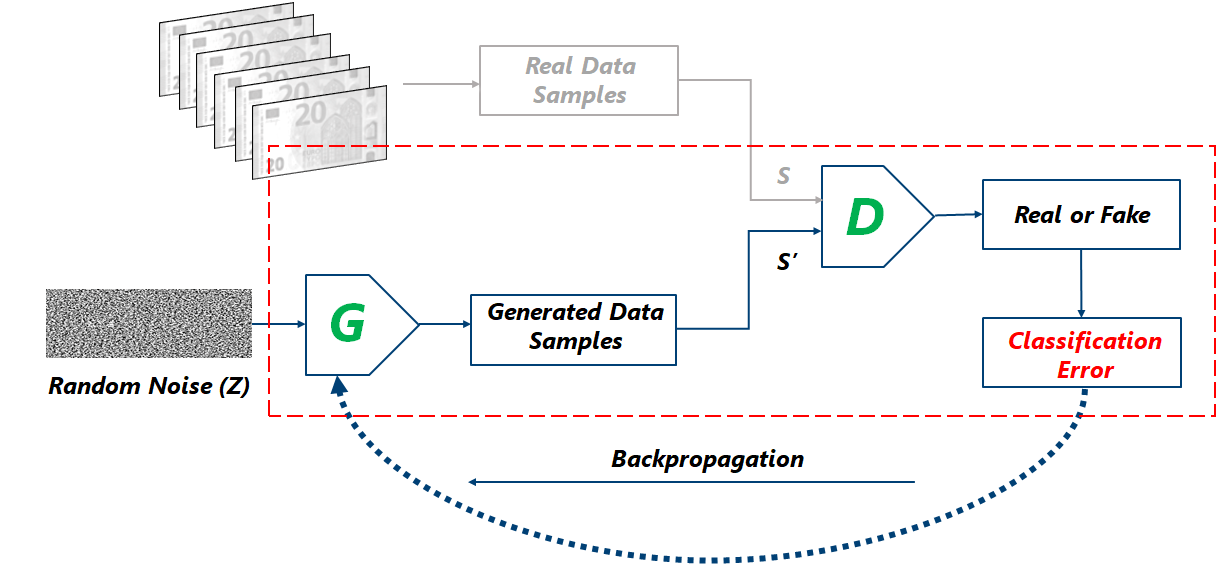
\includegraphics[scale=0.47]{images/Fundamentals/generatorTraining.png}
	\caption[An illustration of the training of the generator $G$ using backpropagation.]{An illustration of the training of the generator $G$ using backpropagation.}
	\label{fig:generatorTraining}
	\end{center}
\end{figure}




\subsubsection{\ac{GAN} Training Algorithm}

\begin{algorithm}[H]
\For{each training iteration}{
 \BlankLine
 \BlankLine
 \BlankLine
	\textbf{1. Train the Discriminator:}
	\BlankLine
	\BlankLine
		\Indp
		a) Get a real data sample $S$ from the training dataset. \\
		\BlankLine
		b) Get a noise vector $Z$ from the random noise distribution, pass it thorough the generator $G$ and create a fake sample $S'$. \\
		\BlankLine
		c) Classify $S$ and $S'$ using the discriminator $D$.\\
		\BlankLine
		d) Backpropagate the calculated classification error to update the discriminator’s weights to minimize classification error.\\
	\BlankLine
	\BlankLine
	\BlankLine
	\Indm
	\textbf{2. Train the Generator:}
	\BlankLine
	\BlankLine
		\Indp
		a) Get a noise vector $Z$ from the random noise distribution, pass it thorough the generator $G$ and create a fake sample $S'$. \\
		\BlankLine
		b) Classify $S'$ using the discriminator $D$.\\
		\BlankLine
		c) Backpropagate the calculated classification error to update the generator’s weights to maximize the discriminator’s error.\\
\BlankLine
\BlankLine
\BlankLine
}	
\caption{\ac{GAN} training algorithm \cite{langr2019gans}.}
\label{alg:ganTrainingAlg}
\end{algorithm}




\newpage
\section{Convolution Neural Networks}\label{CNNs}

In recent years deep learning is evolved with the rise of \acp{ANN}. \acp{ANN} are biologically inspired and capable to solve complex problems \cite{oshea2015introduction}. \acp{CNN} is the most successful image-driven pattern recognition technique among \acp{ANN} \cite{oshea2015introduction}. Nowadays, \acp{CNN} are used to solve difficult image recognition, image classification and object detection tasks. The \acp{CNN} have been a popular method because of its extraordinary results at object recognition competition known as the \ac{ILSVRC} in 2012 for solving computer vision tasks. \ac{CNN} is a kind of deep learning technique for processing data that has a grid pattern, for example, images and videos. \acp{CNN} are inspired by the early findings in the study of biological vision, especially, organization of the animal visual cortex \cite{Hubel.1968} \cite{Fukushima.1980} \cite{10.5555/3153997} and designed to automatically and adaptively learn spatial hierarchies of features, from low-level to high-level patterns \cite{10.5555/3153997}. It is composed of various building blocks, such as convolution layers, pooling layers and fully connected layers. As shown in figure \ref{fig:CNNBuildingBlocks}, the first two layers are convolution and pooling layers and they perform feature extraction. Whereas the third, a fully connected layer, maps the extracted and downsampled features from the convolution layers and pooling layers into the final output, such as probabilities for classification tasks \cite{articleCNNs}. Let's have a look at each layer in the following sections.

%In recent years in the field of machine learning, drastic improvements have occurred to increase the performance of machine learning models. Also, numerous deep learning techniques like \acp{ANN} are evolved significantly.
%These biologically inspired neural networks were able to exceed the performance compared to the traditional machine learning techniques to solve complex problems \cite{oshea2015introduction}. 


\vspace*{0.3cm}
\begin{figure}[H]
        \begin{center}
	    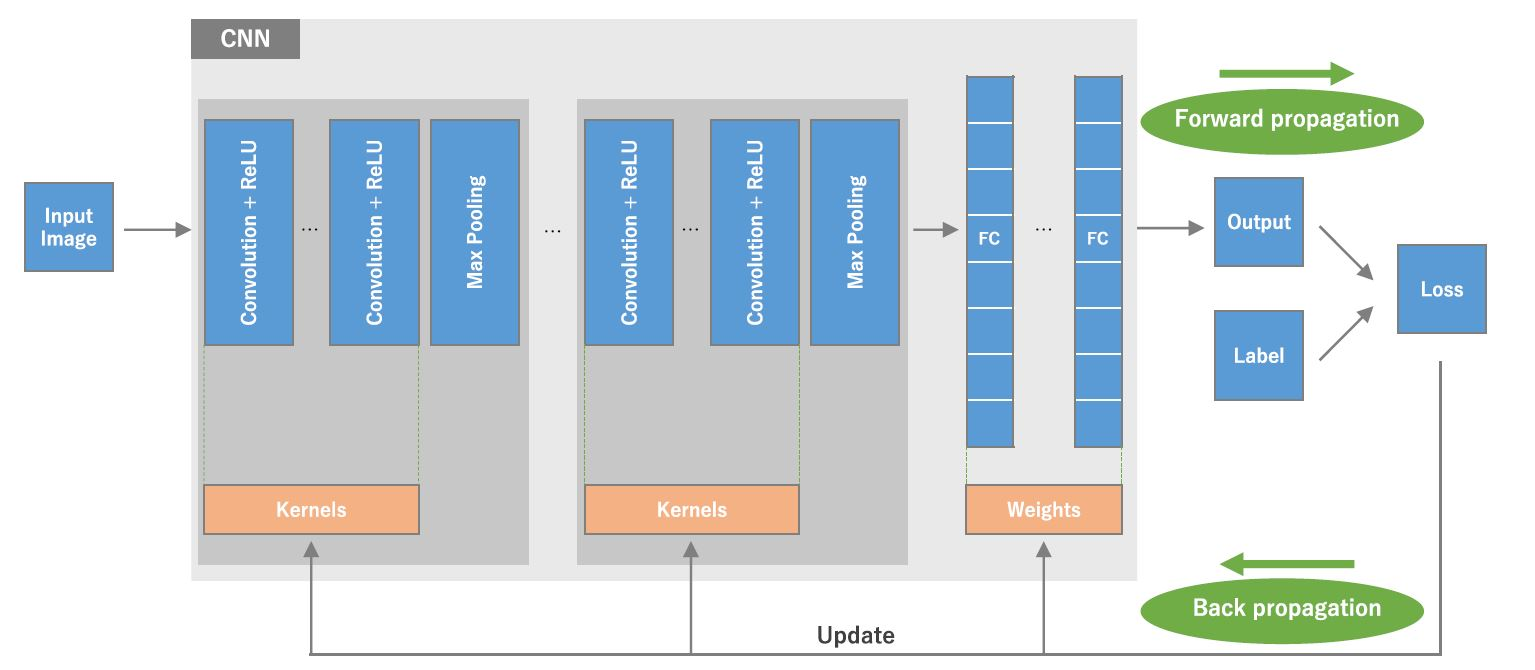
\includegraphics[scale=0.59]{images/Fundamentals/CNNBuildingBlocks.JPG}
	    \caption[An illustration of \ac{CNN} architecture and its training process.]{An illustration of \ac{CNN} architecture and its training process. Convolution layers, pooling layers and fully connected layers are the basic building blocks of \ac{CNN}. These layers are combined to build complex \ac{CNN} architectures to solve different types of problems. These building blocks are stacked upon each other. The \ac{CNN} is trained using the training dataset and the input data is fed into the network in a forward direction. The process of feeding data in the forward direction to the \ac{CNN} is called forward propagation. Each layer receives the input data and processes it through an activation function such as \ac{ReLU} (figure \ref{fig:ActivationFunctions}), then sends it on to the next successive layer. The model's performance is improved by updating the learnable parameters, weights and kernels using the loss value through backpropagation with gradient descent optimization algorithm \cite{ruder2017overview} \cite{articleCNNs}.}
	    \label{fig:CNNBuildingBlocks}
	    \end{center}
\end{figure}





\subsection{Convolution Layer}
The convolution layer is a basic component of the \ac{CNN} that performs feature extraction. It is typically a combination of linear and nonlinear operations like convolution operation and activation function \cite{articleCNNs}. It is one of the core building blocks of \acp{CNN}. Also, it computes for most heavy and complex computations. A convolution layer performs mathematical operations like convolution, a specialized type of linear operation \cite{articleCNNs}. The digital images store pixel values in a \ac{2D} grid, i.e., an array of numbers as shown in figure \ref{fig:Convolution}. The features from an image are extracted using a filter or kernel. A kernel is a small array of numbers applied across an input image, covering all pixels, using a given stride size. As features could exist at any location, the kernel is slid across an input, to perform an element-wise dot product between kernel elements and the input tensor, which is an array of pixel values. An element-wise dot product is performed between kernel's elements and an input tensor and results are added to obtain an output value at the corresponding location of the output tensor, such output tensor is called a feature map (figure \ref{fig:Convolution}a-c) \cite{articleCNNs}. This process extracts all vital features present in an image, making \ac{CNN} highly efficient for image processing and feature extraction tasks \cite{articleCNNs}.

%The layers are connected, one layer feeds its output to the next layer. ``The extracted features can hierarchically and progressively become more complex'' \cite{articleCNNs}. ``Training is the process of optimizing parameters such as kernels optimizing weights of the neurons in \acp{CNN}, which minimizes the difference between outputs and ground truth labels through an optimization algorithm backpropagation and gradient descent'' \cite{Goodfellow-et-al-2016} \cite{ruder2017overview} \cite{articleCNNs}.

\begin{figure}[H]
        \begin{center}
	    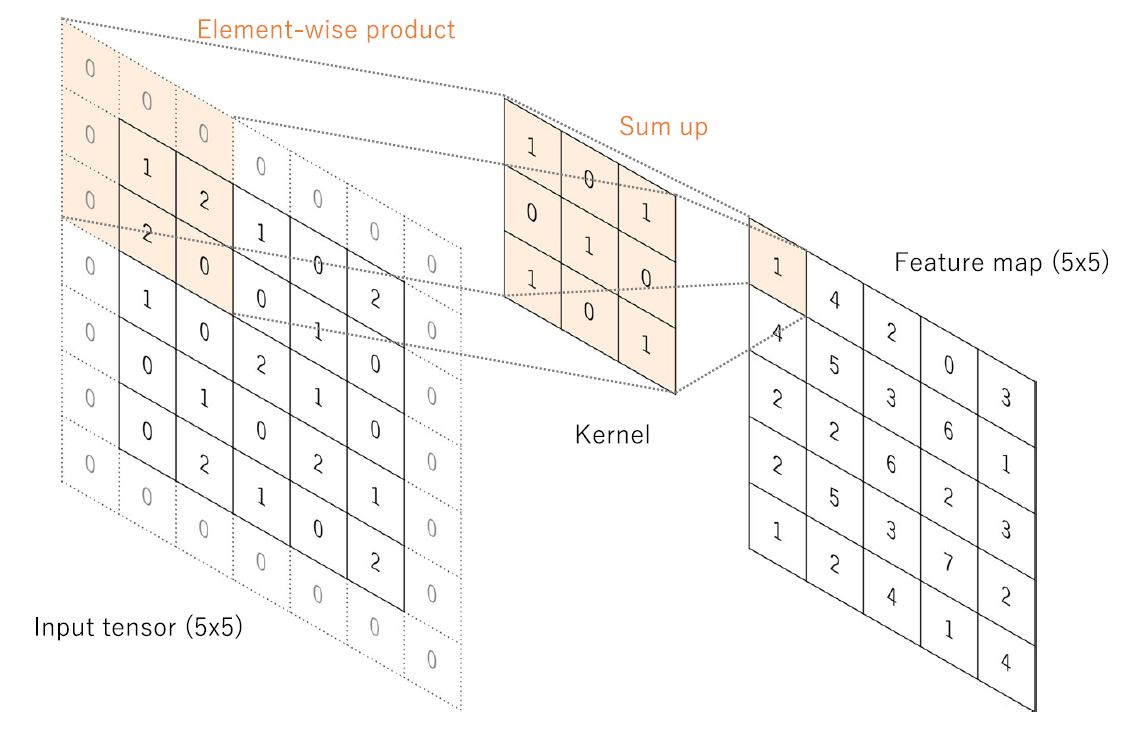
\includegraphics[scale=0.60]{images/Fundamentals/ConvolutionZeroPadding.JPG}
	    \caption[A Convolution Operation With Zero Padding.]{An illustration of a convolution operation with zero padding to retain spatial dimensions. Note that an input dimension of $5 \times 5$ is retained in the generated output feature map. In this example, kernel size is set to $3 \times 3$ and stride is set to $1$ \cite{articleCNNs}.}
	    \label{fig:ConvolutionZeroPadding}
	    \end{center}
\end{figure}

%``For feature extraction linear operation, convolution is used, where a small array of numbers, called a kernel, is applied across the input, which is an array of numbers, called a tensor. An element-wise product between the input tensor and kernel's each element is calculated at each location of the tensor and added to obtain the output value in the corresponding position of the output tensor, called a feature map (figure \ref{fig:Convolution}a-c)'' \cite{articleCNNs}. 

This procedure is repeated by applying multiple kernels to create an arbitrary number of feature maps, which describe different characteristics of the input tensors \cite{articleCNNs}. The different kernels act as separate feature extractors. Two important hyperparameters that represent the convolution operation are the size and number of kernels \cite{articleCNNs}. The size is typically 3 × 3, but sometimes 5 × 5 or 7 × 7, depends on the requirement. The number of kernels is arbitrary and determines the depth of output feature maps. The above-mentioned convolution operation prevents the center of each kernel from overlapping the input tensor's outermost element. Hence, the output feature map's height and width are reduced compared to the input tensor \cite{articleCNNs}. This problem is solved by the zero-padding. In this technique, extra rows and columns of zeros are added around the input tensor so that the kernel's center element overlaps with an outermost element of an input tensor. Zero padding helps to preserve the original spatial dimension throughout convolution operation (figure \ref{fig:ConvolutionZeroPadding}) \cite{articleCNNs}. Modern \ac{CNN} architectures normally employ zero padding to retain spatial dimensions to apply more further layers. Each successive feature map would get smaller after the successive convolution operation without zero padding. A stride is the distance between two successive kernel positions and it also defines the convolution operation \cite{articleCNNs}. A stride of 1 is the most common choice; however, a stride greater than 1 is sometimes used to achieve feature map downsampling. A pooling operation is an alternative technique for downsampling. It is described briefly in section \ref{PoolingLayer}.

\begin{figure}[H]
        \begin{center}
	    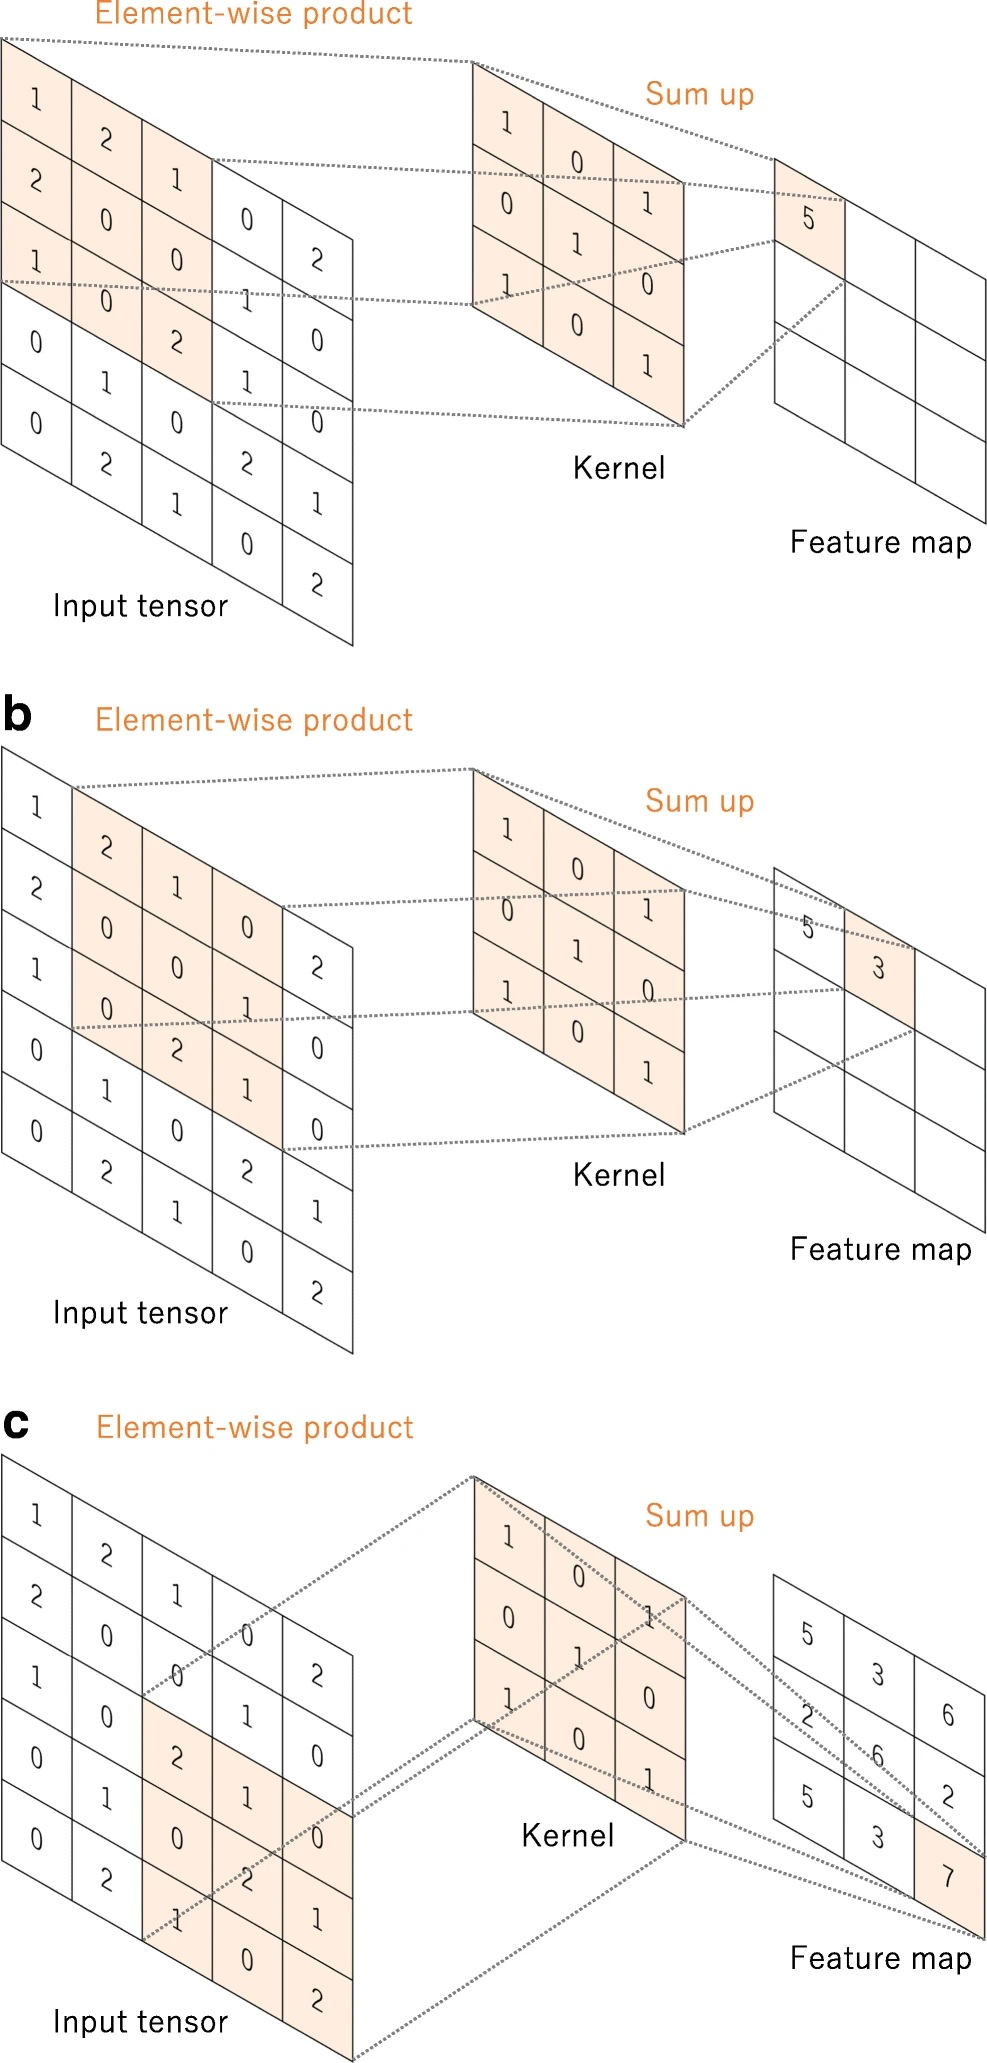
\includegraphics[scale=0.40]{images/Fundamentals/Convolution.JPG}
	    \caption[An illustration of Convolution Operation.]{\textbf{a–c} An illustration of convolution operation with no padding, kernel size $3 \times 3$ and stride $1$ \cite{articleCNNs}.}
	    
	    %A kernel is applied across the input tensor and an element-wise product between each element of the kernel and the input tensor is calculated at each location and summed to obtain the output value in the corresponding position of the output tensor, called a feature map
	    \label{fig:Convolution}
	    \end{center}
\end{figure}


\subsubsection{Activation Functions}


%The \acp{ANN} are inspired by biological neural networks present in the animal brain. Before constructing any \ac{ANN}, it is important to understand the artificial neuron model. In the figure \ref{fig:artificialNeuron} schematic diagram of an artificial neuron is illustrated. 
%A biological neuron gets excited when other neurons with different weights send electrical signals to it. The value of the electrical signal should be big enough to excite the neuron, otherwise, it will be in an inactive state. 
%The addition unit gets the linear weight sum $Z$ of the inputs and bias.
%The brain receives the stimulus from the external world. It processes the information and generates an output. A biological neuron gets excited when other neurons with different weights send electrical signals to it. The value of the electrical signal should be big enough to excite the neuron otherwise, it will be in an inactive state. It learns complex patterns by communicating with millions of neurons inside the brain. The artificial neurons work similarly to biological neurons. 

The artificial neuron is a mathematical function inspired by the neurons inside the brain and they are the basis of \acp{ANN}. The artificial neurons receive one or more weighted inputs and bias, and their sum is passed through an activation function. An artificial neuron's schematic diagram is illustrated in figure \ref{fig:artificialNeuron}, where $\{X_1, X_2, X_3, ..., X_n\}$ are the inputs to the artificial neuron, $\{W_1, W_2, W_3, ..., W_n\}$ are the weights corresponding to the inputs and $b$ is the bias. The summation symbol represents the addition unit. Inputs are fed to the neuron, they perform a linear transformation on these inputs using the weights and biases. If $X = [X_1, X_2, X_3, ..., X_n]  \in R^{n}$  and  $W = [W_1, W_2, W_3, ..., W_n] \in R^{n}$, then output $Z$ is represented as

\begin{equation}\label{linearRegression}
Z=X{W}^\intercal + b.
\end{equation}

\begin{figure}[H]
        \begin{center}
	    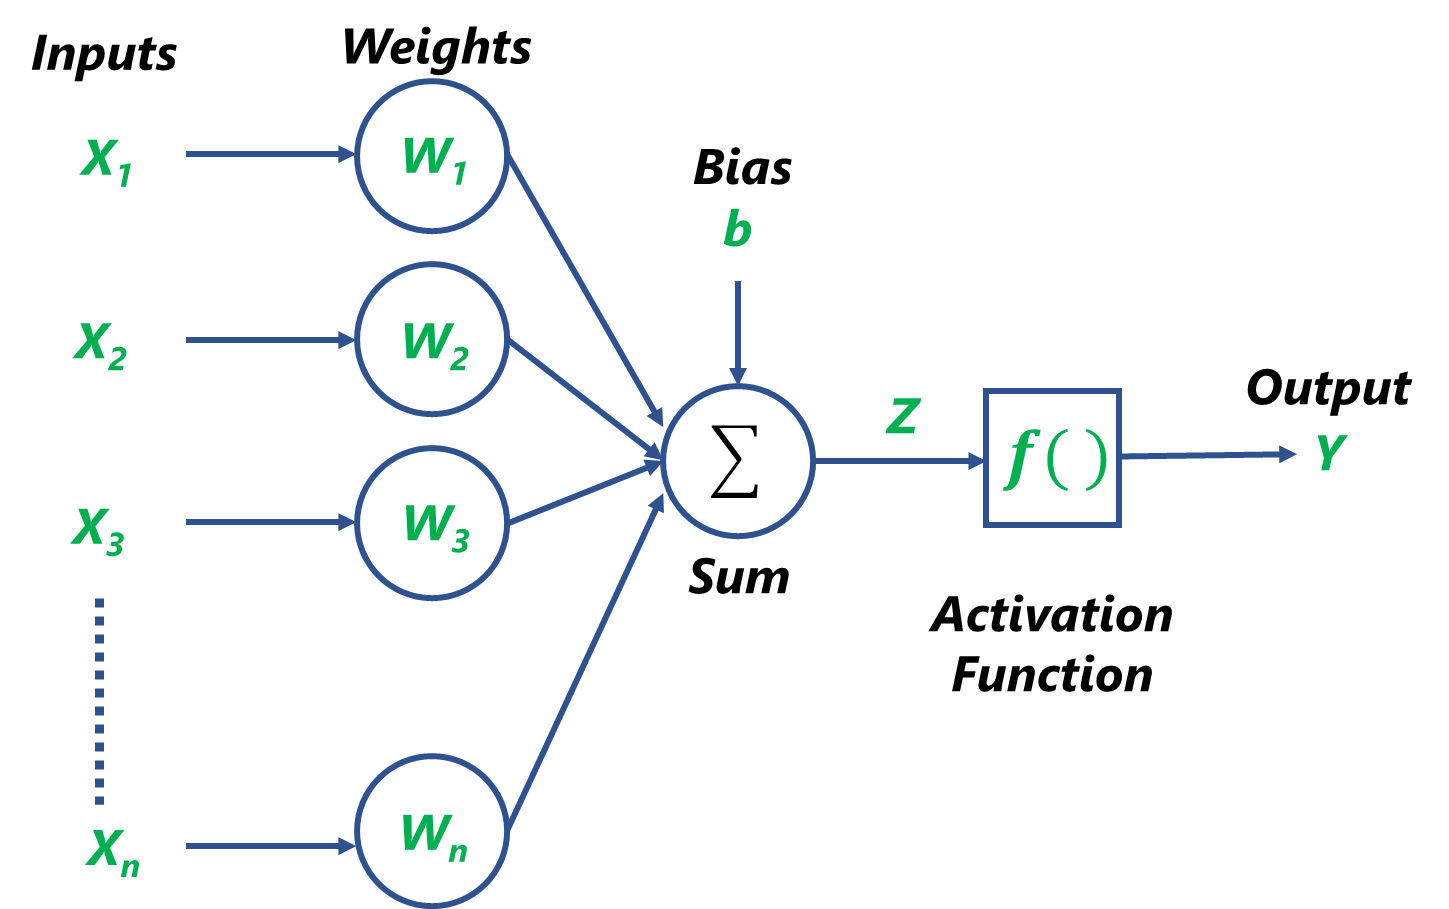
\includegraphics[scale=0.30]{images/Fundamentals/artificialNeuron.png}
	    \caption[An illustration of artificial neuron.]{An illustration of artificial neuron.}
	    \label{fig:artificialNeuron}
	    \end{center}
\end{figure}

The function $f$ is the activation function applied on $Z$.
\begin{equation}\label{artificialNeuron}
Y = f(Z).
\end{equation}

%The activation functions are important while constructing any neural network as they are mathematical functions attached to the neurons. The activation function is applied to the outputs of a linear operation like convolution. Also, they tell which of the neuron is excited or triggered in each layer of neural networks. 
%The main purpose of the activation function is to introduce non-linearity in the neural network. The equation \ref{linearRegression} performs a linear operation. This linear function gets repeated every hidden layer of the neural network. A combination of such linear functions also a linear function, equivalent to all the hidden layers collapsed into a single linear function performing linear regression. Hence, all the hidden layers become useless. Even if linear functions are easy to use, but they fail to learn complex patterns present in the data like images, speech and videos. Hence, nonlinear activation functions are used, while constructing neural networks. 

The data is fed to the input layer of the neurons in neural network, undergoes the linear operation, later, activation functions are applied in the hidden layers and output is produced. The produced output the propagated forward to next hidden layers, this is movement is called forward propagation\footnotemark. In neural networks the hidden layer lies between input layer and output layer. A simple neural network is illustrated in figure \ref{fig:ann}. The main purpose of the activation function is to introduce non-linearity in the neural network. The linear functions are easy to use, but they fail to learn complex patterns present in the data like images, speech and videos. Hence, nonlinear activation functions are used, while constructing neural networks. The nonlinear activation functions are differentiable. The neural networks learn from the errors calculated at the output layer, a differentiable nonlinear activation function is required to perform backpropagation to compute loss with respect to the weights of the neurons and optimize them using gradient descent optimization algorithm or any other optimization algorithm. 

\footnotetext{\url{https://www.analyticsvidhya.com/blog/2020/01/fundamentals-deep-learning-activation-functions-when-to-use-them/} last access: \dcdate}

\begin{figure}[H]
        \begin{center}
	    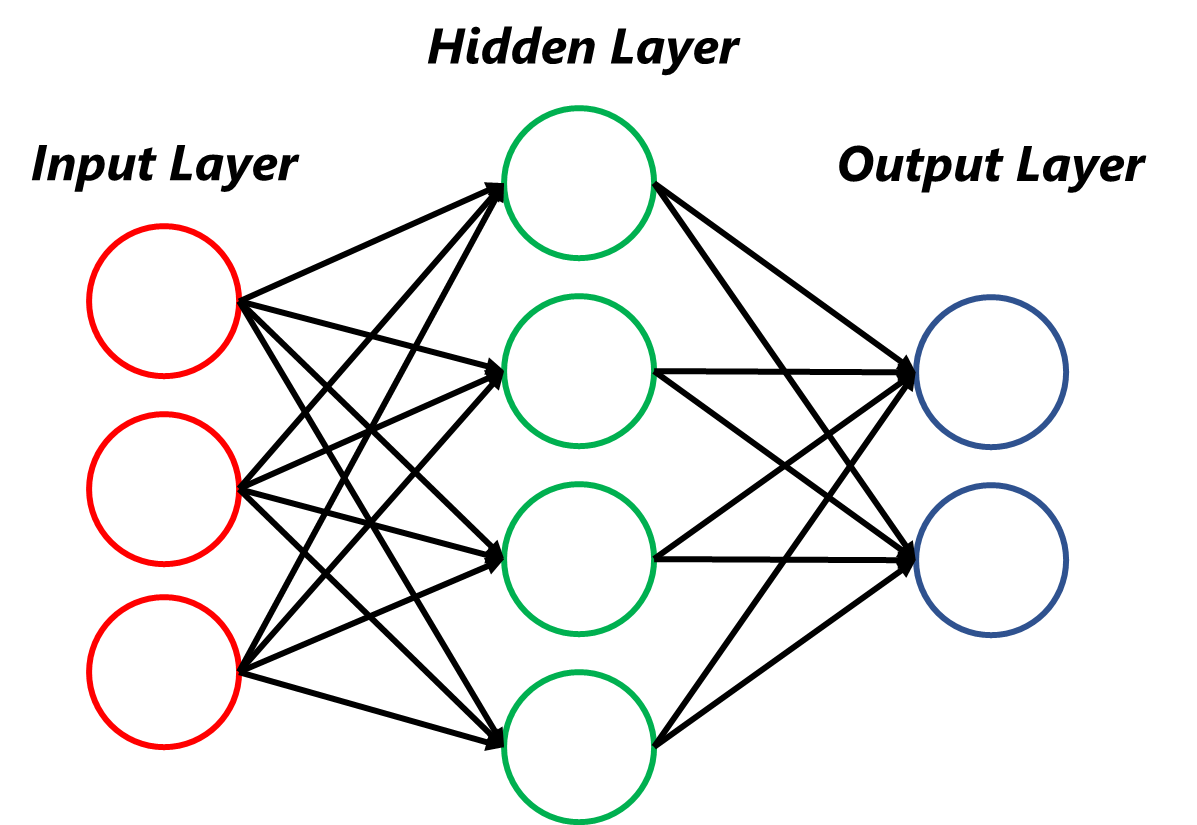
\includegraphics[scale=0.30]{images/Fundamentals/ann.png}
	    \caption[Simple neural network.]{Simple neural network}
	    \label{fig:ann}
	    \end{center}
\end{figure}

The backpropagation minimizes the error, updates the weights of neurons and enhances the accuracy and performance of the neural network. The nonlinear functions, sigmoid, hyperbolic tangent(tanh) functions ware mathematical representations of biological neuron behavior. The \ac{ReLU} is now the most commonly used nonlinear activation function, it computes the function: $f(x) = \max(0, x)$. These activation functions along with their plots are illustrated in figure \ref{fig:ActivationFunctions} \cite{LeCun.2015} \cite{NIPS2012_c399862d}.


% \cite{10.5555/3104322.3104425} \cite{ramachandran2017searching} \cite{pmlr-v15-glorot11a}.



\vspace*{0.5cm}

\begin{figure}[H]
        \begin{center}
	    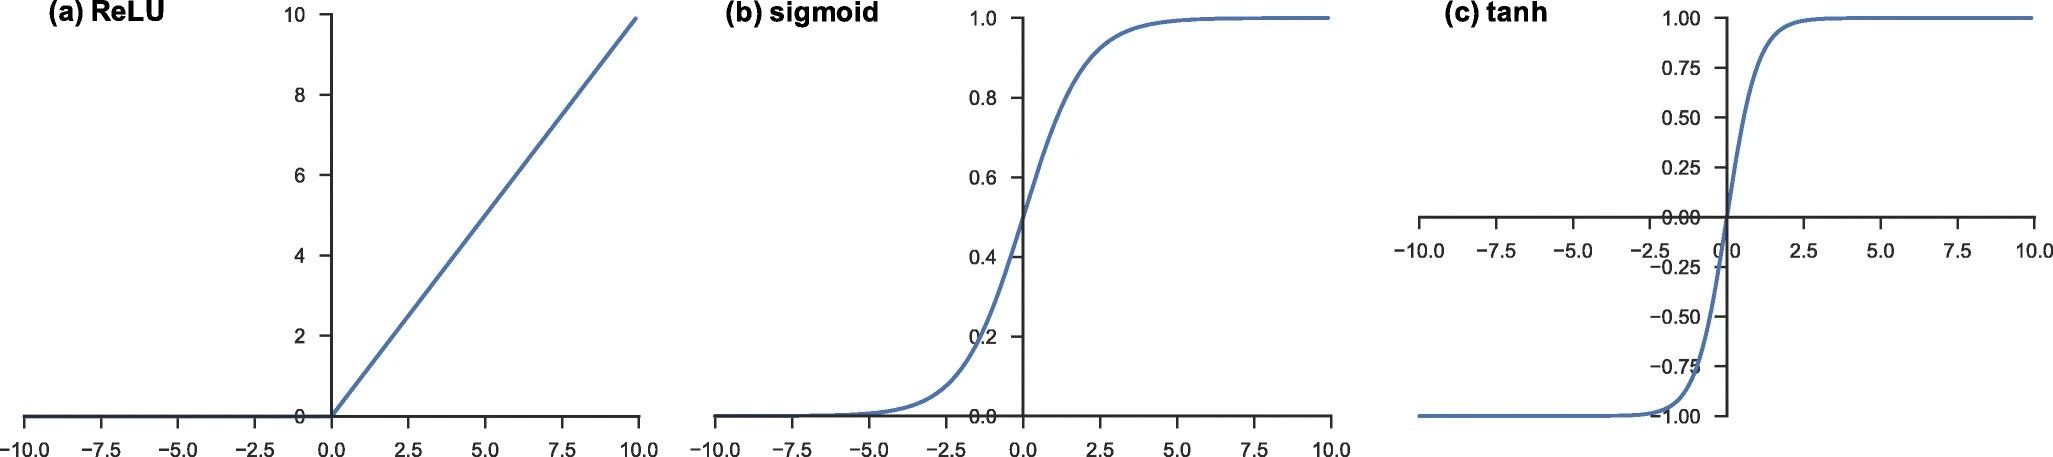
\includegraphics[scale=0.42]{images/Fundamentals/ActivationFunctions.jpg}
	    \caption[Most common nonlinear activation functions used while constructing Neural Networks.]{Most common nonlinear activation functions used while constructing neural networks: \textbf{a)} \ac{ReLU}, \textbf{b)} sigmoid and \textbf{c)} hyperbolic tangent (tanh) \cite{articleCNNs}.}
	    \label{fig:ActivationFunctions}
	    \end{center}
\end{figure}

\subsection{Pooling Layer}\label{PoolingLayer}
A pooling layer performs downsampling on feature maps to gradually reducing the spatial dimensionality, which leads to the reduction of the computational complexity and number of parameters of the neural network and controlling overfitting. Downsampling introduces translation invariance to minor shifts and distortions \cite{goodfellow2017deep}. Downsampling of feature maps can also be accomplished by using convolution layers by increasing the stride of the convolution operation across the image. But the robust and common approach of downsampling is to use a pooling layer \cite{goodfellow2017deep}. Similar to convolution operations, it uses hyperparameters like filter size, stride and padding. Also, it is common to periodically insert a pooling layer in between successive convolution layers while constructing neural networks. There two common types of pooling methods one is max pooling the other is average pooling. The max-pooling considers the most activated (maximum) value in each input patch of the feature map. The average pooling averages values in each input patch of the feature map \cite{10.1007/978-3-642-15825-4_10}.

\subsubsection{Max Pooling}
Max pooling is the most common and popular type of pooling operation. The max-pooling operation is independently operated at every depth slice of the input and resized spatially. Commonly, max-pooling filters are of size $2 \times 2$ and applied with a stride of 2. The max-pooling operation extracts small patches of given filter size from the input feature maps and outputs the maximum value in every patch discarding others (figure \ref{fig:PoolingLayer}) \cite{goodfellow2017deep}. The spatial dimension of feature maps is reduced by a factor of two by discarding 75\% of its activations \cite{kumar2018ordinal}. The height and width dimension of the features maps is reduced but the depth dimension remains unchanged. Pooling operations with larger filter sizes are too destructive and it's worth noting that max-pooling layers do not have learnable parameters \cite{articleCNNs}.


\begin{figure}[H]
        \begin{center}
	    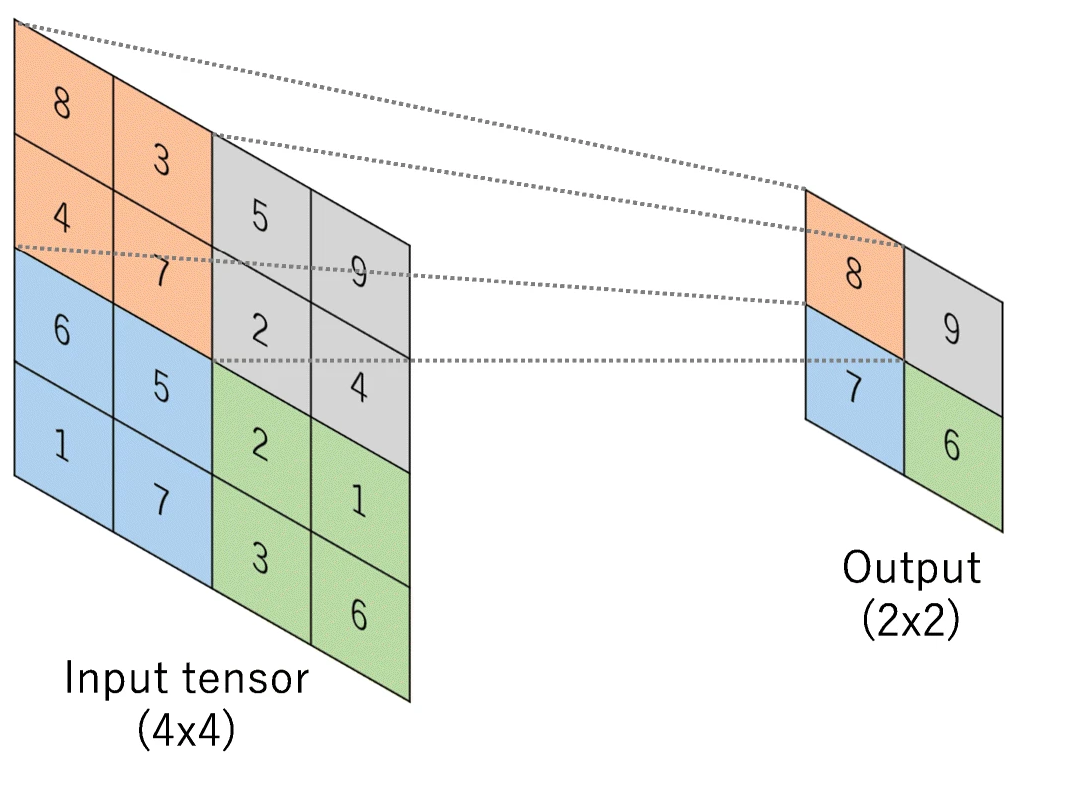
\includegraphics[scale=0.50]{images/Fundamentals/PoolingLayer.png}
	    \caption[An illustration of Max Pooling Operation.]{An illustration of max pooling operation with a filter size of $2 \times 2$, no padding and stride 2. Max pooling operation extracts $2 \times 2$ patches from the input tensors and outputs the maximum value in each patch by ignoring the remaining values. The spatial dimension of an input tensor is downsampled by a factor of 2 \cite{articleCNNs}.}
	    \label{fig:PoolingLayer}
	    \end{center}
\end{figure}


\subsubsection{Global Average Pooling}
There is another type of pooling operation called global average pooling. It performs an extreme type of downsampling. It downsamples a feature map of size $height\ \times width\ \times\ depth$ into a $1\ \times 1\ \times\ depth$ array by averaging all the elements present in the feature map by keeping depth dimension unchanged. This operation is applied only once before fully connected layers. There are some benefits of using global average pooling: a)  It reduces the number of learnable parameters. b) allows the \ac{CNN} to consider inputs of variable size \cite{articleCNNs} \cite{lin2014network}. c) It is intended to replace fully connected layers, the idea is to generate one feature map for each class, in the classification task, as they provide robust spatial information and the resulting vector can easily be fed to the softmax layer\footnotemark.

\footnotetext{\url{https://paperswithcode.com/method/global-average-pooling/} last access: \dcdate}





\subsection{Fully connected layer}

%In neural networks, ``fully connected layers are those layers where all the inputs from one layer are connected to every neuron of the next layer'' \cite{articleCNNs}. 

The final output feature map of convolution layers or pooling layers is flattened and the output is transformed into a \ac{1D} vector. The flattened output is connected to one or more fully connected layers. The fully connected layers are also called dense layers, where every input is connected to every output by a learnable weight \cite{articleCNNs}. A fully connected layer performs multiplication between the input and weight matrix then adds a bias vector \cite{articleCNNs}. Equation \ref{artificialNeuron} represents the task of each neuron in a fully connected layer. Each fully connected layer is followed by a nonlinear activation function, for example, \ac{ReLU}. As already described, the nonlinear activation function helps neurons learn complex patterns. The features present in an image are extracted using convolution layers and downsampled by pooling layers. Next, extracted features are mapped through fully connected layers to the final output of the neural network, determining the probability for each class in classification tasks. Usually, the number of output nodes in the fully connected layer is equal to the number of classes \cite{articleCNNs}. The last fully connected layer's activation function is usually different than others. Each task chooses a suitable activation function. Often, in binary classification tasks sigmoid activation function is used. For example, logistic regression, models the probabilities for binary classification tasks using the sigmoid activation function\footnotemark. The softmax activation function is widely used in multiclass classification tasks. The output of the last fully connected layers are normalized into target class probabilities by the softmax activation function, in the classification tasks. The probability of each class ranges between 0 and 1 and the sum of all target class probabilities is 1 \cite{articleCNNs}.


\footnotetext{\url{https://machinelearningmastery.com/choose-an-activation-function-for-deep-learning/} last access: \dcdate}






























%%%%%%%%%%%%%%%%%%%%%%%%%%%%%%%%%%%%%%%%%%%%%%%%%%%%%%%%%%%%%%%%%%%%%%%%%%%%%%%%%%%%%%%%%%%%%%%%%%%%%%%%%%%%%%%%%%%%%%%%%%%%%%%%%%%%%%%%%


\begin{comment}
\begin{center}
\begin{table}[H]
    \begin{center}
    \begin{tabular}{p{0.40\linewidth} p{0.40\linewidth}} 
        \toprule
        Task & Last layer activation function \\ %[1.0ex] 
        \midrule
        Binary classification & Sigmoid\\ %[1.0ex] 
        \midrule
        Multiclass single-class classification & Softmax \\ %[1.0ex]
        \midrule
        Multiclass multiclass classification & Sigmoid \\ %[1.0ex]
        \midrule
        Regression to continuous values & Identity \\ %[1.0ex]
        \bottomrule
    \end{tabular}
    \caption{A list of commonly applied last layer activation functions for various tasks.}
    \label{table:activationfunction}
    \end{center}
\end{table}
\end{center}
\end{comment}


%Another pooling operation worth noting is a global average pooling \cite{lin2014network}. An extreme type of downsampling is performed by global average pooling. Eventually, global average pooling downsamples a feature map with a size of height $\times$ width into a $1 \times 1$ array by simply taking the average of all the elements in each feature map while maintaining the depth of feature maps. Before the fully connected layers, this operation is usually applied only once \cite{articleCNNs}. The following are the benefits of using global average pooling: (1) it reduces the number of learnable parameters and (2) it allows the \ac{CNN} to accept inputs of variable size. Before the fully connected layers, this operation is usually performed only once. The following are some of the benefits of using global average pooling: (1) the number of learnable parameters is decreased and (2) allows the CNN to consider inputs of variable size

%In recent years tremendous interest in deep learning has developed. The most successful algorithm among numerous deep learning models is \acp{CNN}. It is a class of artificial neural networks. It has been a prevailing method in solving computer vision tasks since the extraordinary results were shared on the object recognition competition known as the \ac{ILSVRC} in 2012 [ \cite{russakovsky2015imagenet}, \cite{NIPS2012_4824}]. It has been a popular method in solving computer vision tasks since the remarkable performance at the object recognition competition known as the \ac{ILSVRC} in 2012 [ \cite{russakovsky2015imagenet}, \cite{NIPS2012_4824}]. 
%\footnote{A convolution is a mathematical operation that slides one function over another and measures the integral of their pointwise multiplication. It has deep connections with the Fourier transform and the Laplace transform and is heavily used in signal processing. Convolutional layers actually use cross-correlations, which are very similar to convolutions (see \url{https://homl.info/76} for more details) \cite{10.5555/3153997}last access: 08.05.2021.}


%\acp{CNN} combinations of several building blocks like convolution layers, pooling layers (e.g., max pooling, global average pooling) and fully connected layers. These building blocks are stacked on each other. With a loss function through forward propagation on a training dataset, a model’s performance under particular kernels and weights is calculated. The learnable parameters, like kernels and weights, are updated as per the loss value through backpropagation using a gradient descent optimization algorithm \cite{ruder2017overview}. The ReLU notation stands for the rectified linear unit. It is an activation function \ref{fig:ActivationFunctions} \cite{articleCNNs}.

\begin{comment}
\begin{center}
\begin{table}
    \begin{tabular}{p{0.25\linewidth} p{0.15\linewidth} p{0.50\linewidth}} 
        \toprule
        & Parameters & Hyperparameters\\ %[1.0ex] 
        \midrule
        Convolution layer & Kernels & Kernel size, number of kernels, stride, padding, activation function \\ %[1.0ex]
        \midrule
        Pooling layer & None & Pooling method, filter size, stride, padding \\ %[1.0ex]
        \midrule
        Fully connected layer & Weights & Number of weights, activation function \\ %[1.0ex]
        \midrule
        Others & & Model architecture, optimizer, learning rate, loss function, mini-batch size, epochs, regularization, weight initialization, dataset splitting\\% [1.0ex]
        \bottomrule
    \end{tabular}
    \caption{A list of parameters and hyperparameters in a convolutional neural network (\ac{CNN}).}
    \label{table:hyperparametersCNN}
\end{table}
\end{center}
\end{comment}

%Max pooling is the most common form of pooling operation, which extracts patches from the input feature maps, outputs the maximum value in each patch and discards the rest (figure \ref{fig:PoolingLayer}). In practice, a max pooling with a size $2 \times 2$ filter and a stride of 2 is widely used. The spatial dimension of feature maps is reduced by a factor of two. The depth dimension of feature maps, unlike the height and width dimensions, does not change.

\begin{comment}
The discriminator in a \ac{GAN} is a binary classifier. It tries to classify between real data and the data generated by the generator. The discriminator can use any network architecture which is suitable to the kind of data it's classifying. The  training data of the discriminator comes from two sources: a) Real Data Samples. During training, the discriminator uses these samples as positive instances. b) Fake Data Samples generated by the generator. The discriminator uses these samples as negative instances during training. In figure \ref{fig:discriminatorTraining}, the two ``Sample" boxes represent these two data sources feeding into the discriminator.


The generator does not train when the discriminator is training. The generator's weights remain unchanged while it generates samples to train the discriminator. The discriminator is connected to two loss functions. The discriminator completely ignores the generator loss and just uses the discriminator loss during its training. The generator loss is used during generator training to update its weights. The coming section \ref{TheGeneratorSubSection} describes why the generator loss connects to the discriminator. During the discriminator training process: a) Discriminator classifies both real data and fake data generated from the generator. b) The discriminator loss penalizes the discriminator for wrongly classifying a real instance as fake or a fake instance as real. c) Through backpropagation, the discriminator updates its weights using the discriminator loss through the discriminator network.
\end{comment}

\begin{comment}
The generator part of a \ac{GAN} learns to create fake data by receiving backpropagation loss from the discriminator. Slowly it learns and trains to make the discriminator classify its fake output as real. Generator training requires a closer alliance between the generator and the discriminator as compared to the discriminator training requires. The part of the \ac{GAN} that trains the generator includes: a) Random input data. b) Generator network, which transforms the random input data into plausible data. c) Discriminator network, which classifies the generated data. d) Discriminator output. e) Generator loss, which penalizes the generator for failing to fool the discriminator. Neural networks need some form of input data, like an example for classification or to predict about. But what to consider as an input for a neural network that outputs entirely new data instances? In its most fundamental form, a \ac{GAN} takes random noise as its input. The generator then transforms this random noise into a plausible output. By introducing random noise, \ac{GAN} can generate a wide variety of data, sampling from different places in the target distribution. Investigations suggest that the distribution of the noise doesn’t matter much, therefore it is possible to choose something easy to sample from, as a uniform distribution. For simplicity, the distribution from which the noise is sampled is usually of a smaller dimension than the dimensionality of the output distribution. To train a neural network, its weights are updated to reduce the error or loss of its output.  In \ac{GAN}, however, the generator is not directly connected to the loss that is required to update its weights. The discriminator produces the generator loss as the generator feeds into the discriminator network. The generator loss penalizes the generator for generating a sample that the discriminator network classifies as fake. This extra piece of the implementation must be included in backpropagation. The backpropagation adjusts the weights in the appropriate direction by calculating the weight’s impact on the output — how the output would change if you updated the weights. But the impact of a generator weight depends on the discriminator weights it feeds into. So generator loss is backpropagated from the output of the discriminator to the generator. Means gradients flow back through the discriminator into the generator. 


At the same time, the discriminator will not change during generator training. Attempting to hit a moving target would make a complicated problem even difficult for the generator. The generator is trained with the following procedure: 1) Random noise input to the generator. 2) Generator produces output from sampled random noise. 3) The discriminator determines whether the generator output is “Real” or “Fake”. 4) Calculate loss from discriminator classification. 5) Backpropagate the generator loss through both the discriminator and generator to obtain gradients. 6) Use the gradients to update only the generator's weights.
\end{comment}

\begin{comment}
The \ac{GAN} has two training models one is a generator and another is a discriminator. The generator learns to generate plausible data. The discriminator always aims to reject samples produced by the generator as the generated samples are negative training samples for the discriminator. Throughout the training, the discriminator learns to distinguish the generator's fake data from real data. When the generator produces implausible results the discriminator penalizes it. Once the training starts, the generator generates fake data and the discriminator learns to rejects the data by saying the generator that it's fake data. As training progresses, the generator learns to produce the output that can fool the discriminator. Lastly, if generator training is successful, the discriminator gets bad at telling the difference between real data and fake data generated by the generator. The discriminator starts to classify fake data as real and its accuracy decreases. Ultimately, the generator will start producing plausible data. Both the generator and the discriminator are neural networks. The generator's output is connected directly to the discriminator's input. The discriminator's classification provides the loss that the generator uses to update its weights using backpropagation.

\subsection{The Discriminator}\label{TheDiscriminatorSubSection}

\vspace*{-0.7cm}
\begin{figure}[H]
        \begin{center}
	    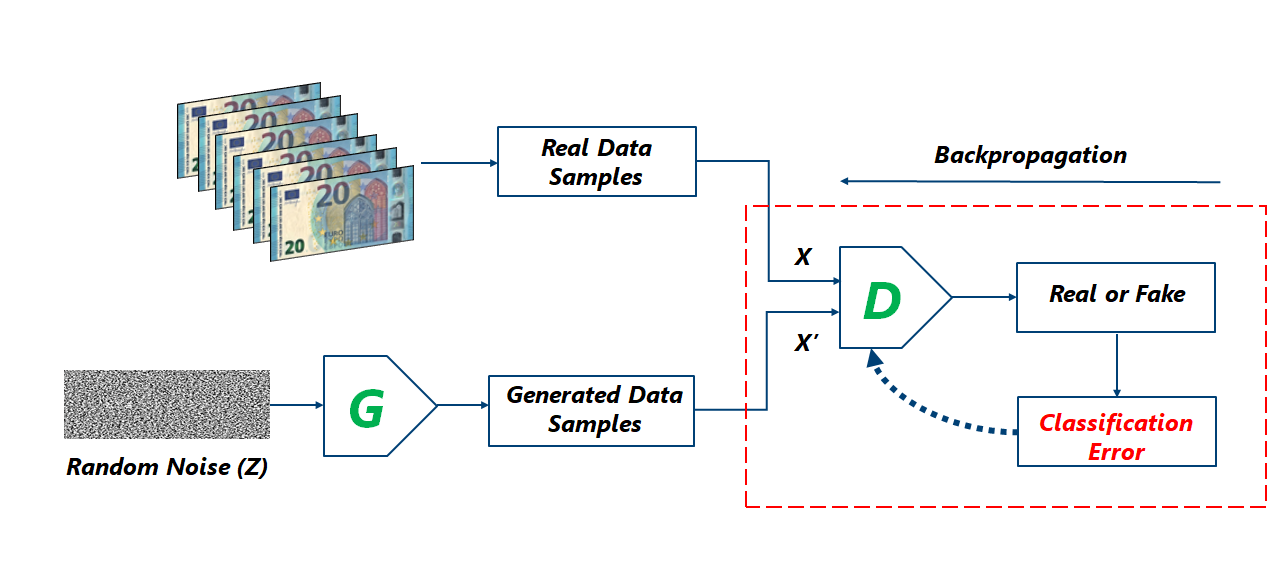
\includegraphics[scale=0.45]{images/discriminatorTraining.png}
	    \caption[Illustartion of the training of the discriminator $D$ using backpropagation.]{Training of the discriminator $D$ using backpropagation.}
	    \label{fig:discriminatorTraining}
	    \end{center}
\end{figure}

The discriminator in a \ac{GAN} is a binary classifier. It tries to classify between real data and the data generated by the generator. The discriminator can use any network architecture which is suitable to the kind of data it's classifying. The  training data of the discriminator comes from two sources: a) Real Data Samples. During training, the discriminator uses these samples as positive instances. b) Fake Data Samples generated by the generator. The discriminator uses these samples as negative instances during training. In figure \ref{fig:discriminatorTraining}, the two ``Sample" boxes represent these two data sources feeding into the discriminator. The generator does not train when the discriminator is training. The generator's weights remain unchanged while it generates samples to train the discriminator. The discriminator is connected to two loss functions. The discriminator completely ignores the generator loss and just uses the discriminator loss during its training. The generator loss is used during generator training to update its weights. The coming section \ref{TheGeneratorSubSection} describes why the generator loss connects to the discriminator. During the discriminator training process: a) Discriminator classifies both real data and fake data generated from the generator. b) The discriminator loss penalizes the discriminator for wrongly classifying a real instance as fake or a fake instance as real. c) Through backpropagation, the discriminator updates its weights using the discriminator loss through the discriminator network.





\subsection{The Generator}\label{TheGeneratorSubSection}

%\vspace*{1.5cm}
\begin{figure}[H]
    \begin{center}
	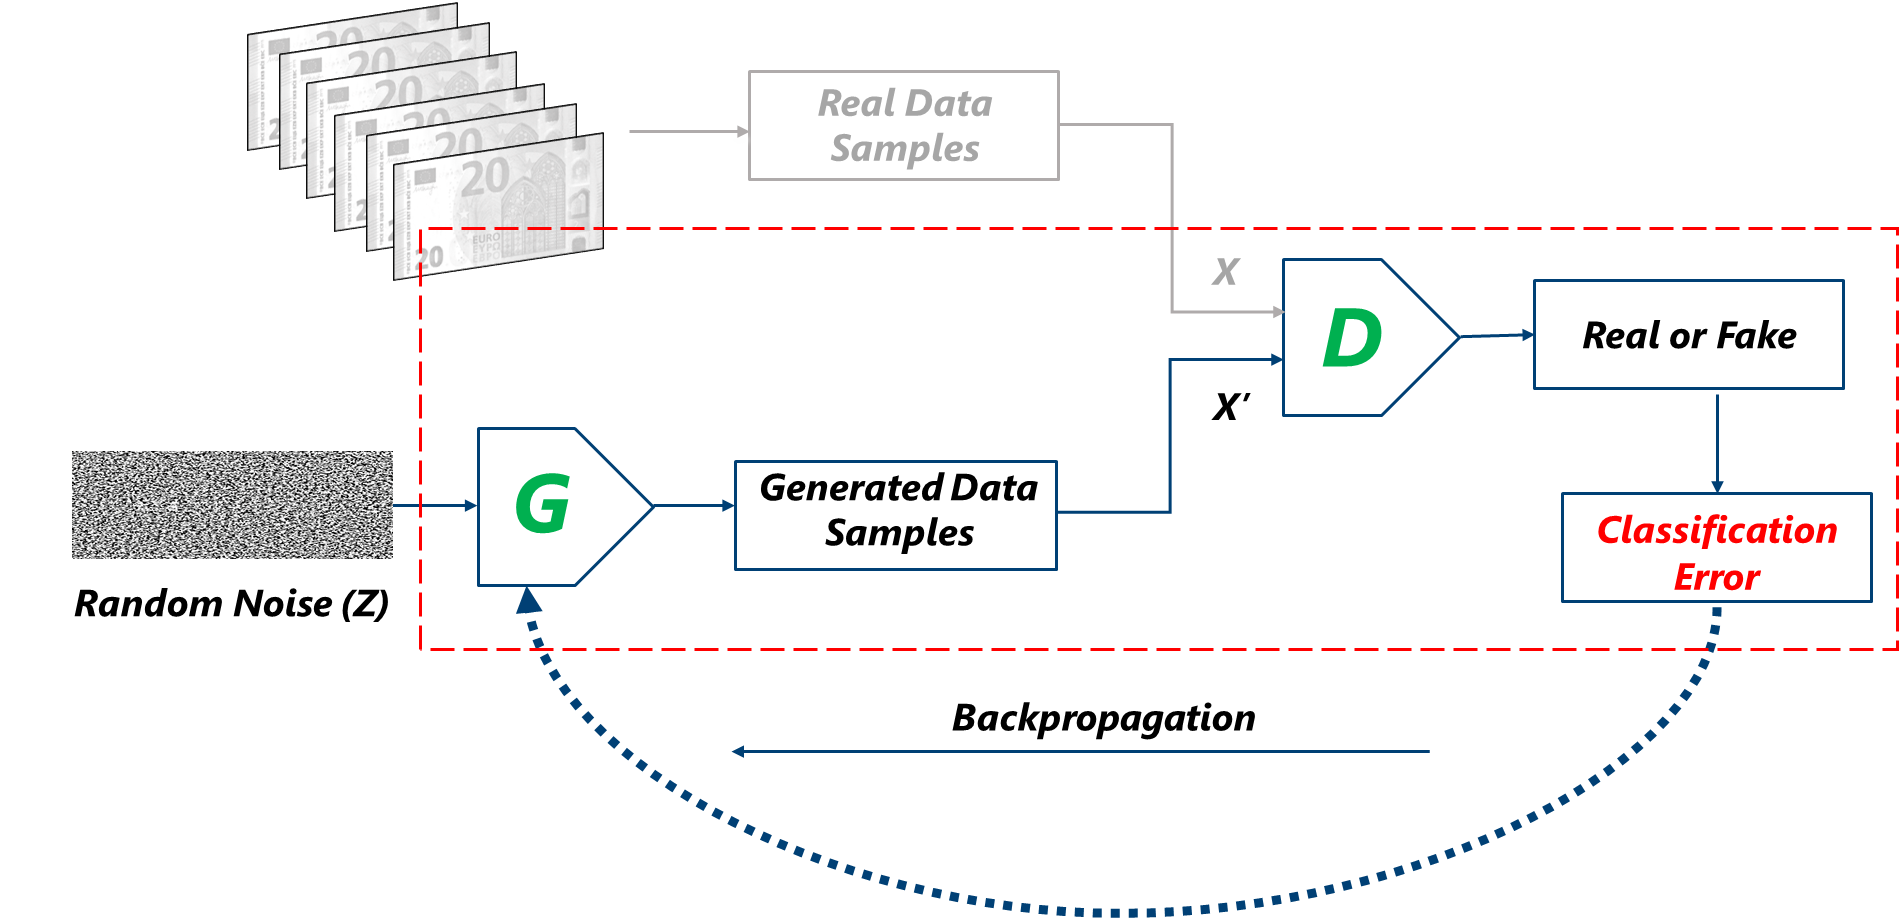
\includegraphics[scale=0.30]{images/generatorTraining.png}
	\caption[Training Generator $G$ using backpropagation]{Training Generator $G$ using backpropagation.}
	\label{fig:generatorTraining}
	\end{center}
\end{figure}

The generator part of a \ac{GAN} learns to create fake data by receiving backpropagation loss from the discriminator. Slowly it learns and trains to make the discriminator classify its fake output as real. Generator training requires a closer alliance between the generator and the discriminator as compared to the discriminator training requires. The part of the \ac{GAN} that trains the generator includes: a) Random input data. b) Generator network, which transforms the random input data into plausible data. c) Discriminator network, which classifies the generated data. d) Discriminator output. e) Generator loss, which penalizes the generator for failing to fool the discriminator. Neural networks need some form of input data, like an example for classification or to predict about. But what to consider as an input for a neural network that outputs entirely new data instances? In its most fundamental form, a \ac{GAN} takes random noise as its input. The generator then transforms this random noise into a plausible output. By introducing random noise, \ac{GAN} can generate a wide variety of data, sampling from different places in the target distribution. Investigations suggest that the distribution of the noise doesn’t matter much, therefore it is possible to choose something easy to sample from, as a uniform distribution. For simplicity, the distribution from which the noise is sampled is usually of a smaller dimension than the dimensionality of the output distribution. To train a neural network, its weights are updated to reduce the error or loss of its output.  In \ac{GAN}, however, the generator is not directly connected to the loss that is required to update its weights. The discriminator produces the generator loss as the generator feeds into the discriminator network. The generator loss penalizes the generator for generating a sample that the discriminator network classifies as fake. This extra piece of the implementation must be included in backpropagation. The backpropagation adjusts the weights in the appropriate direction by calculating the weight’s impact on the output — how the output would change if you updated the weights. But the impact of a generator weight depends on the discriminator weights it feeds into. So generator loss is backpropagated from the output of the discriminator to the generator. Means gradients flow back through the discriminator into the generator. At the same time, the discriminator will not change during generator training. Attempting to hit a moving target would make a complicated problem even difficult for the generator. The generator is trained with the following procedure: 1) Random noise input to the generator. 2) Generator produces output from sampled random noise. 3) The discriminator determines whether the generator output is “Real” or “Fake”. 4) Calculate loss from discriminator classification. 5) Backpropagate the generator loss through both the discriminator and generator to obtain gradients. 6) Use the gradients to update only the generator's weights.

\end{comment}

